\section{Physical Represenatations}
\label{sec:physical}

We developed several in-memory representations of evolving graphs to
explore the trade-offs of compactness, parallelism, and support of
different query operators. \eat{ The data structures represent a
  continuum of replication, from the SnapshotGraph to OneGraph and are
  described here in more detail.}

{\bf SnapshotGraph (SG).} The simplest way to represent an evolving
graph is by representing each snapshot individually, a direct
translation of our logical data model.  We call this data structure
SnapshotGraph, or SG for short. An example of an SG is depicted in
Figure~\ref{fig:sgp}.  SG is a collection of snapshots, where vertices
and edges store the attribute values for the specific time interval.
A \insql{TSelect} operation on this representation is a slice of the
snapshot sequence, while \insql{TGroup} and temporal joins
(\insql{TAnd} and \insql{TOr}) require a group by key within each
aggregate set of vertices and edges.

\begin{figure}[t!]
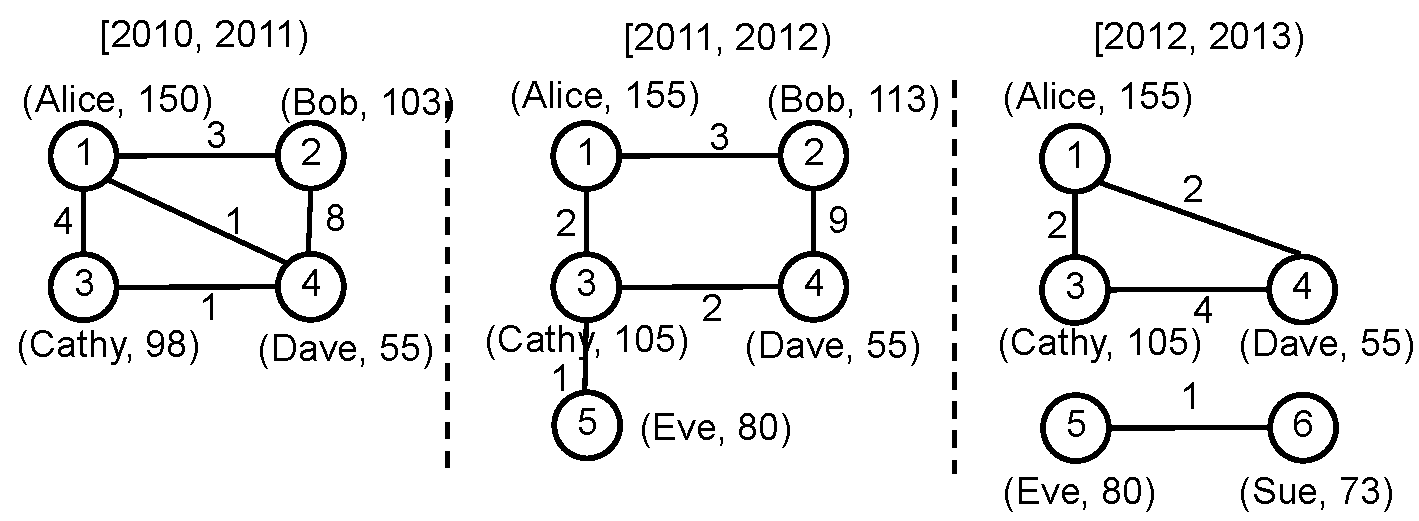
\includegraphics[width=3.2in]{figs/sgp.pdf}
\caption{SG representation of T1 from Figure~\ref{fig:tg}.}
\label{fig:sgp}
\end{figure}

While the SG representation is simple, it is not compact, considering
that in many real-world evolving graphs there is a 80\% or larger
similarity between consecutive
snapshots~\cite{DBLP:journals/tos/MiaoHLWYZPCC15}.  In a distributed
architecture, however, this data structure provides some benefits as
operations on it can be easily parallelized, by assigning different
snapshots to different workers, or by partitioning a snapshot across
workers.  

{\bf OneGraphColumn (OGC).}  The most topologically compact
representation of graph structure is to store each vertex {\em and}
each edge only once for the whole evolving graph, by taking a union of
the snapshot vertex and edge sets.  The OneGraphColumn data structure,
or OGC for short, uses this representation in our system. 

The OGC data structure provides some benefits in addition to
compactness, since it reduces the total communication between vertices
in Pregel-based analytics in batch mode.  The drawback is that OGC is
much denser than individual snapshots of SG.  OGC stores vertex and
edge attribute information separately.  This is not as compact as
storing attributes within the graph elements, but is faster in many
operations where only graph topology is required.

\begin{figure}[t!]
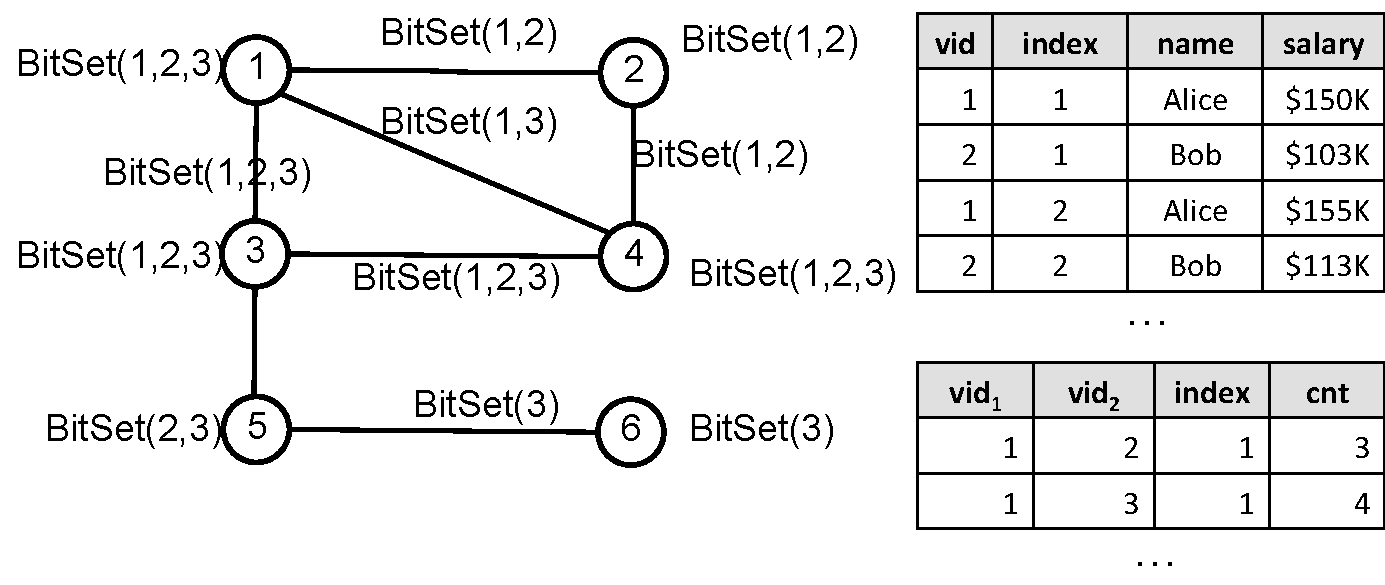
\includegraphics[width=3.2in]{figs/ogc.pdf}
\caption{OGC of T1 from~\ref{fig:tg}.}
\label{fig:ogc}
\end{figure}


{\bf Third data structure}

{\bf Partitioning, briefly.}
